%--------------------------------------------------------------
% thesis.tex 
%--------------------------------------------------------------
% Corso di Laurea in Informatica 
% http://if.dsi.unifi.it/
% @Facolt\`a di Scienze Matematiche, Fisiche e Naturali
% @Universit\`a degli Studi di Firenze
%--------------------------------------------------------------
% - template for the main file of Informatica@Unifi Thesis 
% - based on Classic Thesis Style Copyright (C) 2008 
%   Andr\'e Miede http://www.miede.de   
%--------------------------------------------------------------
\documentclass[twoside,openright,titlepage,fleqn,
	headinclude,12pt,a4paper,BCOR5mm,footinclude]{scrbook}
%--------------------------------------------------------------
\newcommand{\myItalianTitle}{Super Risoluzione\xspace}
\newcommand{\myEnglishTitle}{SuperRes\xspace}
% use the right myDegree option
\newcommand{\myDegree}{Corso di Laurea in Informatica\xspace}
%\newcommand{\myDegree}{
	%Corso di Laurea Specialistica in Scienze e Tecnologie 
	%dell'Informazione\xspace}
\newcommand{\myName}{Filippo Mameli\xspace}
\newcommand{\myProf}{Marco Bertini\xspace}
\newcommand{\myOtherProf}{Correlatore\xspace}
\newcommand{\mySupervisor}{Nome Cognome\xspace}
\newcommand{\myFaculty}{
	Scuola di Scienze Matematiche, Fisiche e Naturali\xspace}
\newcommand{\myUni}{\protect{
	Universit\`a degli Studi di Firenze}\xspace}
\newcommand{\myLocation}{Firenze\xspace}
\newcommand{\myTime}{Anno Accademico 2018-2019\xspace}
\newcommand{\myVersion}{Version 0.1\xspace}
%--------------------------------------------------------------
\usepackage[italian]{babel}
\usepackage[latin1]{inputenc} 
\usepackage[T1]{fontenc} 
\usepackage[square,numbers]{natbib} 
\usepackage[fleqn]{amsmath}  
\usepackage{ellipsis}
\usepackage{listings}
\usepackage{subfig}
\usepackage{caption}
\usepackage{appendix}
\usepackage{siunitx}
%--------------------------------------------------------------
\usepackage{dia-classicthesis-ldpkg}
%--------------------------------------------------------------
% Options for classicthesis.sty:
% tocaligned eulerchapternumbers drafting linedheaders 
% listsseparated subfig nochapters beramono eulermath parts 
% minionpro pdfspacing
\usepackage[eulerchapternumbers,linedheaders,subfig,beramono,eulermath,
parts]{classicthesis}
%--------------------------------------------------------------
\newlength{\abcd} % for ab..z string length calculation
% how all the floats will be aligned
\newcommand{\myfloatalign}{\centering} 
\setlength{\extrarowheight}{3pt} % increase table row height
\captionsetup{format=hang,font=small}
%--------------------------------------------------------------
% Layout setting
%--------------------------------------------------------------
\usepackage{geometry}
\geometry{
	a4paper,
	ignoremp,
	bindingoffset = 1cm, 
	textwidth     = 13.5cm,
	textheight    = 21.5cm,
	lmargin       = 3.5cm, % left margin
	tmargin       = 4cm    % top margin 
}

\lstset{
  	frame=tb,
	language=Matlab,
  	aboveskip=3mm,
  	belowskip=3mm,
  	showstringspaces=false,
  	columns=flexible,
  	basicstyle={\small\ttfamily},
  	numbers=none,
  	breaklines=true,
  	breakatwhitespace=true,
  	tabsize=3
}
%--------------------------------------------------------------
\begin{document}
\frenchspacing
\raggedbottom
\pagenumbering{roman}
\pagestyle{plain}
%--------------------------------------------------------------
% Frontmatter
%--------------------------------------------------------------
%--------------------------------------------------------------
% titlepage.tex (use thesis.tex as main file)
%--------------------------------------------------------------
\begin{titlepage}
	\begin{center}
   	\large
      \hfill
      \vfill
      \begingroup
         
\includegraphics[scale=0.15]{logo/LOGO}\\
%			\spacedallcaps{\myUni} \\ 
			\myFaculty \\
			\myDegree \\ 
			\vspace{0.5cm}
         \vspace{0.5cm}    
         Tesi di Laurea    
      \endgroup 
      \vfill 
      \begingroup
      	\color{Maroon}\spacedallcaps{\myItalianTitle} \\ $\ $\\
      	\spacedallcaps{\myEnglishTitle} \\ 	
	\bigskip
      \endgroup
      \spacedlowsmallcaps{\myName}
      \vfill 
      \vfill
      Relatore: \emph{Relatore}\\
      Correlatore: \emph{Correlatore}\\
      \vfill
      \vfill
      \myTime
      \vfill                      
	\end{center}        
\end{titlepage}   
%--------------------------------------------------------------
% back titlepage
%--------------------------------------------------------------
   \newpage
	\thispagestyle{empty}
	\hfill
	\vfill
	\noindent\myName: 
	\textit{\myItalianTitle,} 
	\myDegree, \textcopyright\ \myTime
%--------------------------------------------------------------
% back titlepage end
%--------------------------------------------------------------
\pagestyle{scrheadings}
%--------------------------------------------------------------
% Mainmatter
%--------------------------------------------------------------
\pagenumbering{arabic}
% use \cleardoublepage here to avoid problems with pdfbookmark
%\include{intro} % use \myChapter command instead of \chapter
% \tableofcontents
% \listoffigures
% \cleardoublepage
% \thispagestyle{empty}
% \begin{flushright}
% \null\vspace{\stretch {1}}
% \emph{"Inserire citazione" \break --- Inserire autore citazione} \vspace{\stretch{2}}\null
% \end{flushright}
% \cleardoublepage
\chapter{Risultati}

\section{Metriche}

\begin{tabular}{lllll}
            & SSIM   & LPIPS  & BRISQUE Out & NIQE Out \\
LPIPS Patch & 0.7443 & 0.1726 & 89.95       & 17.90    \\
MSE         & 0.69   & 0.1462 & 85.98       & 16.68    \\
SSIM loss   & 0.6919 & 0.1933 & 84.74       & 17.55    \\
Target      &        &        & 85.32       & 15.69   
\end{tabular}

\begin{figure}[h]
      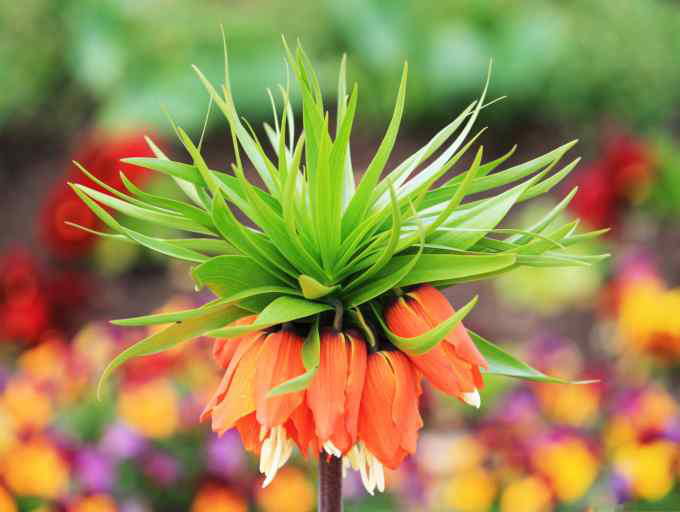
\includegraphics[scale=0.5]{img/flower_512_validation.png}
      \caption{Immagine di partenza}
      \centering
\end{figure}

\begin{figure}[h]
      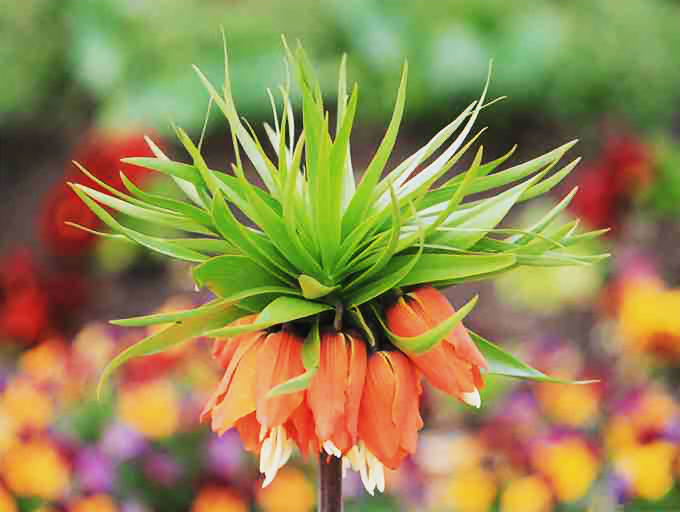
\includegraphics[scale=0.5]{img/flower_512_MSE.png}
      \caption{Immagine generata usando MSE loss}
      \centering
\end{figure}


\begin{figure}[h]
      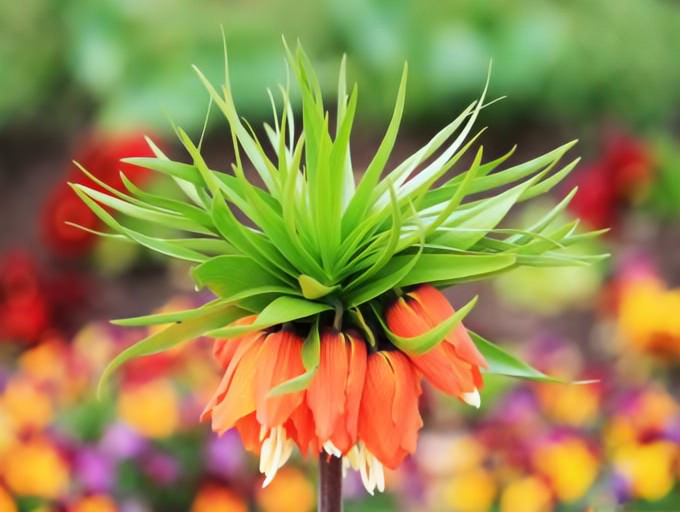
\includegraphics[scale=0.5]{img/flower_512_patches64px.png}
      \caption{Immagine generata usando LPIPS loss su patch}
      \centering
\end{figure}

% \begin{figure}[h]
%       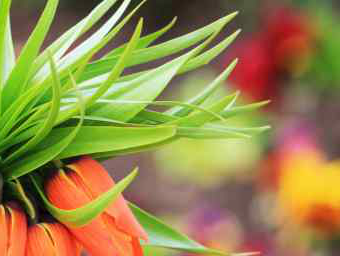
\includegraphics[scale=1.0]{img/flower_512_validation_crop.png}
%       \caption{Crop dell'immagine di partenza}
%       \centering
% \end{figure}

\begin{figure}[h]
      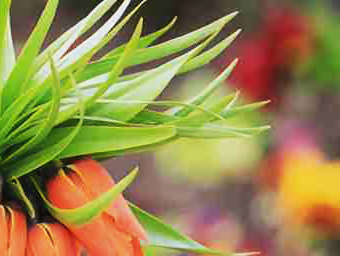
\includegraphics[scale=1.0]{img/flower_512_MSE_crop.png}
      \caption{Crop dell'immagine generata usando MSE loss}
      \centering
\end{figure}

\begin{figure}[h]
      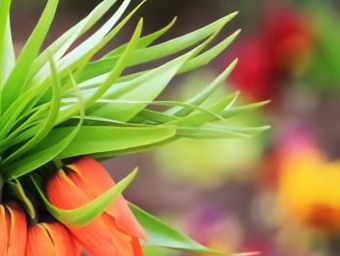
\includegraphics[ scale=1.0]{img/flower_512_patches64px_crop.png}
      \caption{Crop dell'immagine generata usando LPIPS loss su patch}
      \centering
\end{figure}
\begin{thebibliography}{99}

\bibitem{etichetta1}{Autore - \emph{titolo}}

\bibitem{etichetta2}{Autore - \emph{Titolo} - altre informazioni}

\end{thebibliography}

%--------------------------------------------------------------
\end{document}
%--------------------------------------------------------------
